% Created by tikzDevice version 0.12.3.1 on 2021-09-17 14:36:51
% !TEX encoding = UTF-8 Unicode
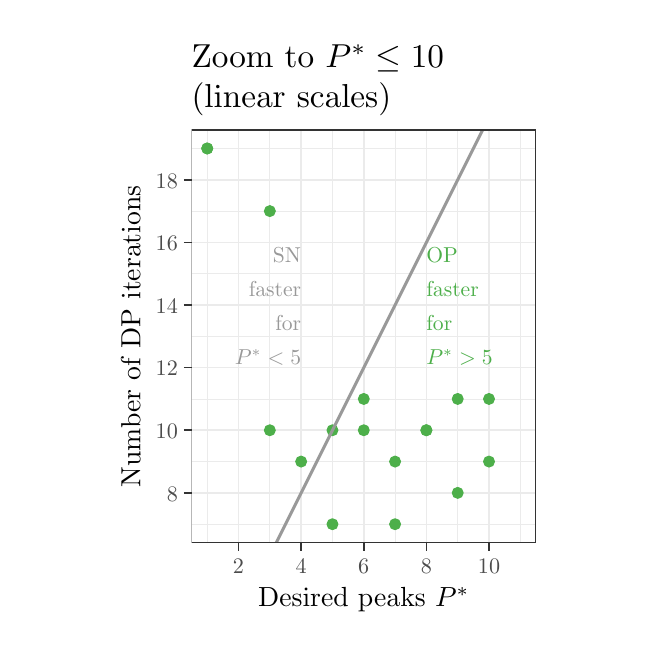
\begin{tikzpicture}[x=1pt,y=1pt]
\definecolor{fillColor}{RGB}{255,255,255}
\path[use as bounding box,fill=fillColor,fill opacity=0.00] (0,0) rectangle (216.81,216.81);
\begin{scope}
\path[clip] ( 27.64,  0.00) rectangle (189.17,216.81);
\definecolor{drawColor}{RGB}{255,255,255}
\definecolor{fillColor}{RGB}{255,255,255}

\path[draw=drawColor,line width= 0.6pt,line join=round,line cap=round,fill=fillColor] ( 27.64,  0.00) rectangle (189.17,216.81);
\end{scope}
\begin{scope}
\path[clip] ( 59.22, 30.61) rectangle (183.67,179.95);
\definecolor{fillColor}{RGB}{255,255,255}

\path[fill=fillColor] ( 59.22, 30.61) rectangle (183.67,179.95);
\definecolor{drawColor}{gray}{0.92}

\path[draw=drawColor,line width= 0.3pt,line join=round] ( 59.22, 37.39) --
	(183.67, 37.39);

\path[draw=drawColor,line width= 0.3pt,line join=round] ( 59.22, 60.02) --
	(183.67, 60.02);

\path[draw=drawColor,line width= 0.3pt,line join=round] ( 59.22, 82.65) --
	(183.67, 82.65);

\path[draw=drawColor,line width= 0.3pt,line join=round] ( 59.22,105.28) --
	(183.67,105.28);

\path[draw=drawColor,line width= 0.3pt,line join=round] ( 59.22,127.91) --
	(183.67,127.91);

\path[draw=drawColor,line width= 0.3pt,line join=round] ( 59.22,150.53) --
	(183.67,150.53);

\path[draw=drawColor,line width= 0.3pt,line join=round] ( 59.22,173.16) --
	(183.67,173.16);

\path[draw=drawColor,line width= 0.3pt,line join=round] ( 64.88, 30.61) --
	( 64.88,179.95);

\path[draw=drawColor,line width= 0.3pt,line join=round] ( 87.50, 30.61) --
	( 87.50,179.95);

\path[draw=drawColor,line width= 0.3pt,line join=round] (110.13, 30.61) --
	(110.13,179.95);

\path[draw=drawColor,line width= 0.3pt,line join=round] (132.76, 30.61) --
	(132.76,179.95);

\path[draw=drawColor,line width= 0.3pt,line join=round] (155.39, 30.61) --
	(155.39,179.95);

\path[draw=drawColor,line width= 0.3pt,line join=round] (178.01, 30.61) --
	(178.01,179.95);

\path[draw=drawColor,line width= 0.6pt,line join=round] ( 59.22, 48.71) --
	(183.67, 48.71);

\path[draw=drawColor,line width= 0.6pt,line join=round] ( 59.22, 71.34) --
	(183.67, 71.34);

\path[draw=drawColor,line width= 0.6pt,line join=round] ( 59.22, 93.96) --
	(183.67, 93.96);

\path[draw=drawColor,line width= 0.6pt,line join=round] ( 59.22,116.59) --
	(183.67,116.59);

\path[draw=drawColor,line width= 0.6pt,line join=round] ( 59.22,139.22) --
	(183.67,139.22);

\path[draw=drawColor,line width= 0.6pt,line join=round] ( 59.22,161.85) --
	(183.67,161.85);

\path[draw=drawColor,line width= 0.6pt,line join=round] ( 76.19, 30.61) --
	( 76.19,179.95);

\path[draw=drawColor,line width= 0.6pt,line join=round] ( 98.82, 30.61) --
	( 98.82,179.95);

\path[draw=drawColor,line width= 0.6pt,line join=round] (121.45, 30.61) --
	(121.45,179.95);

\path[draw=drawColor,line width= 0.6pt,line join=round] (144.07, 30.61) --
	(144.07,179.95);

\path[draw=drawColor,line width= 0.6pt,line join=round] (166.70, 30.61) --
	(166.70,179.95);
\definecolor{drawColor}{RGB}{77,175,74}
\definecolor{fillColor}{RGB}{77,175,74}

\path[draw=drawColor,line width= 0.4pt,line join=round,line cap=round,fill=fillColor] ( 64.88,173.16) circle (  1.96);

\path[draw=drawColor,line width= 0.4pt,line join=round,line cap=round,fill=fillColor] ( 87.50, 71.34) circle (  1.96);

\path[draw=drawColor,line width= 0.4pt,line join=round,line cap=round,fill=fillColor] ( 98.82, 60.02) circle (  1.96);

\path[draw=drawColor,line width= 0.4pt,line join=round,line cap=round,fill=fillColor] (110.13, 71.34) circle (  1.96);

\path[draw=drawColor,line width= 0.4pt,line join=round,line cap=round,fill=fillColor] (121.45, 82.65) circle (  1.96);

\path[draw=drawColor,line width= 0.4pt,line join=round,line cap=round,fill=fillColor] (132.76, 37.39) circle (  1.96);

\path[draw=drawColor,line width= 0.4pt,line join=round,line cap=round,fill=fillColor] (144.07, 71.34) circle (  1.96);

\path[draw=drawColor,line width= 0.4pt,line join=round,line cap=round,fill=fillColor] (155.39, 82.65) circle (  1.96);

\path[draw=drawColor,line width= 0.4pt,line join=round,line cap=round,fill=fillColor] (166.70, 60.02) circle (  1.96);

\path[draw=drawColor,line width= 0.4pt,line join=round,line cap=round,fill=fillColor] ( 64.88,173.16) circle (  1.96);

\path[draw=drawColor,line width= 0.4pt,line join=round,line cap=round,fill=fillColor] ( 87.50,150.53) circle (  1.96);

\path[draw=drawColor,line width= 0.4pt,line join=round,line cap=round,fill=fillColor] (110.13, 37.39) circle (  1.96);

\path[draw=drawColor,line width= 0.4pt,line join=round,line cap=round,fill=fillColor] (121.45, 71.34) circle (  1.96);

\path[draw=drawColor,line width= 0.4pt,line join=round,line cap=round,fill=fillColor] (132.76, 60.02) circle (  1.96);

\path[draw=drawColor,line width= 0.4pt,line join=round,line cap=round,fill=fillColor] (144.07, 71.34) circle (  1.96);

\path[draw=drawColor,line width= 0.4pt,line join=round,line cap=round,fill=fillColor] (155.39, 48.71) circle (  1.96);

\path[draw=drawColor,line width= 0.4pt,line join=round,line cap=round,fill=fillColor] (166.70, 82.65) circle (  1.96);
\definecolor{drawColor}{gray}{0.60}

\path[draw=drawColor,line width= 1.1pt,line join=round] (-65.23,-279.40) -- (308.12,467.32);

\node[text=drawColor,anchor=base east,inner sep=0pt, outer sep=0pt, scale=  0.78] at ( 98.82,132.10) {SN};

\node[text=drawColor,anchor=base east,inner sep=0pt, outer sep=0pt, scale=  0.78] at ( 98.82,119.81) {faster};

\node[text=drawColor,anchor=base east,inner sep=0pt, outer sep=0pt, scale=  0.78] at ( 98.82,107.52) {for};

\node[text=drawColor,anchor=base east,inner sep=0pt, outer sep=0pt, scale=  0.78] at ( 98.82, 95.23) {$P^*<5$};
\definecolor{drawColor}{RGB}{77,175,74}

\node[text=drawColor,anchor=base west,inner sep=0pt, outer sep=0pt, scale=  0.78] at (144.07,132.10) {OP};

\node[text=drawColor,anchor=base west,inner sep=0pt, outer sep=0pt, scale=  0.78] at (144.07,119.81) {faster};

\node[text=drawColor,anchor=base west,inner sep=0pt, outer sep=0pt, scale=  0.78] at (144.07,107.52) {for};

\node[text=drawColor,anchor=base west,inner sep=0pt, outer sep=0pt, scale=  0.78] at (144.07, 95.23) {$P^*>5$};
\definecolor{drawColor}{gray}{0.20}

\path[draw=drawColor,line width= 0.6pt,line join=round,line cap=round] ( 59.22, 30.61) rectangle (183.67,179.95);
\end{scope}
\begin{scope}
\path[clip] (  0.00,  0.00) rectangle (216.81,216.81);
\definecolor{drawColor}{gray}{0.30}

\node[text=drawColor,anchor=base east,inner sep=0pt, outer sep=0pt, scale=  0.80] at ( 54.27, 45.69) {8};

\node[text=drawColor,anchor=base east,inner sep=0pt, outer sep=0pt, scale=  0.80] at ( 54.27, 68.32) {10};

\node[text=drawColor,anchor=base east,inner sep=0pt, outer sep=0pt, scale=  0.80] at ( 54.27, 90.95) {12};

\node[text=drawColor,anchor=base east,inner sep=0pt, outer sep=0pt, scale=  0.80] at ( 54.27,113.58) {14};

\node[text=drawColor,anchor=base east,inner sep=0pt, outer sep=0pt, scale=  0.80] at ( 54.27,136.20) {16};

\node[text=drawColor,anchor=base east,inner sep=0pt, outer sep=0pt, scale=  0.80] at ( 54.27,158.83) {18};
\end{scope}
\begin{scope}
\path[clip] (  0.00,  0.00) rectangle (216.81,216.81);
\definecolor{drawColor}{gray}{0.20}

\path[draw=drawColor,line width= 0.6pt,line join=round] ( 56.47, 48.71) --
	( 59.22, 48.71);

\path[draw=drawColor,line width= 0.6pt,line join=round] ( 56.47, 71.34) --
	( 59.22, 71.34);

\path[draw=drawColor,line width= 0.6pt,line join=round] ( 56.47, 93.96) --
	( 59.22, 93.96);

\path[draw=drawColor,line width= 0.6pt,line join=round] ( 56.47,116.59) --
	( 59.22,116.59);

\path[draw=drawColor,line width= 0.6pt,line join=round] ( 56.47,139.22) --
	( 59.22,139.22);

\path[draw=drawColor,line width= 0.6pt,line join=round] ( 56.47,161.85) --
	( 59.22,161.85);
\end{scope}
\begin{scope}
\path[clip] (  0.00,  0.00) rectangle (216.81,216.81);
\definecolor{drawColor}{gray}{0.20}

\path[draw=drawColor,line width= 0.6pt,line join=round] ( 76.19, 27.86) --
	( 76.19, 30.61);

\path[draw=drawColor,line width= 0.6pt,line join=round] ( 98.82, 27.86) --
	( 98.82, 30.61);

\path[draw=drawColor,line width= 0.6pt,line join=round] (121.45, 27.86) --
	(121.45, 30.61);

\path[draw=drawColor,line width= 0.6pt,line join=round] (144.07, 27.86) --
	(144.07, 30.61);

\path[draw=drawColor,line width= 0.6pt,line join=round] (166.70, 27.86) --
	(166.70, 30.61);
\end{scope}
\begin{scope}
\path[clip] (  0.00,  0.00) rectangle (216.81,216.81);
\definecolor{drawColor}{gray}{0.30}

\node[text=drawColor,anchor=base,inner sep=0pt, outer sep=0pt, scale=  0.80] at ( 76.19, 19.62) {2};

\node[text=drawColor,anchor=base,inner sep=0pt, outer sep=0pt, scale=  0.80] at ( 98.82, 19.62) {4};

\node[text=drawColor,anchor=base,inner sep=0pt, outer sep=0pt, scale=  0.80] at (121.45, 19.62) {6};

\node[text=drawColor,anchor=base,inner sep=0pt, outer sep=0pt, scale=  0.80] at (144.07, 19.62) {8};

\node[text=drawColor,anchor=base,inner sep=0pt, outer sep=0pt, scale=  0.80] at (166.70, 19.62) {10};
\end{scope}
\begin{scope}
\path[clip] (  0.00,  0.00) rectangle (216.81,216.81);
\definecolor{drawColor}{RGB}{0,0,0}

\node[text=drawColor,anchor=base,inner sep=0pt, outer sep=0pt, scale=  1.00] at (121.45,  7.63) {Desired peaks $P^*$};
\end{scope}
\begin{scope}
\path[clip] (  0.00,  0.00) rectangle (216.81,216.81);
\definecolor{drawColor}{RGB}{0,0,0}

\node[text=drawColor,rotate= 90.00,anchor=base,inner sep=0pt, outer sep=0pt, scale=  1.00] at ( 40.68,105.28) {Number of DP iterations};
\end{scope}
\begin{scope}
\path[clip] (  0.00,  0.00) rectangle (216.81,216.81);
\definecolor{drawColor}{RGB}{0,0,0}

\node[text=drawColor,anchor=base west,inner sep=0pt, outer sep=0pt, scale=  1.20] at ( 59.22,202.26) {Zoom to $P^* \leq 10$};

\node[text=drawColor,anchor=base west,inner sep=0pt, outer sep=0pt, scale=  1.20] at ( 59.22,188.00) {(linear scales)};
\end{scope}
\end{tikzpicture}
